% !TeX root = main.tex
\section{ HPL Test and Optimization}
This section presents the analysis and optimization test results of our HPL. 

\subsection{Analysis of HPL}
\ 

The High-Performance Linpack (HPL) Benchmark serves as a standardized computational tool for evaluating the floating-point performance capabilities of HPC systems. 
By solving large-scale systems of linear equations $\mathbf{Ax}{=}\mathbf{b}$, i.e., Eq.\ref{eq:4-1}, where matrix  $\mathbf{A}$ represents an  $n\times n $large-scale dense matrix, this benchmark quantifies system performance in FLOPS. 
This method is one of the internationally recognized standards for assessing supercomputer performance.

One way to solve Eq.\ref{eq:4-1} is Gaussian elimination, which first results in a triangular matrix by first converting the $\mathbf{A}$ in the $\mathbf{Ax}{=}\mathbf{b}$ equation into a triangular matrix by elimination.

Suppose the solution problem is
\begin{equation}
\begin{bmatrix}
a_{11} & a_{12} & \cdots & a_{1n} \\
a_{21} & a_{22} & \cdots & a_{2n} \\
\vdots & \vdots & \ddots & \vdots \\
a_{n1} & a_{n2} & \cdots & a_{nn}
\end{bmatrix}
\begin{bmatrix}
x_1 \\ x_2 \\ \vdots \\ x_n
\end{bmatrix}
=
\begin{bmatrix}
b_1 \\ b_2 \\ \vdots \\ b_n
\end{bmatrix}
\label{eq:4-1}
\end{equation}

The basic idea of solving the equation about $\mathbf{x}$ is as follows. 
First, the matrix transformation of $\mathbf{A}$ is carried out to obtain the following form:
\begin{equation}
\begin{bmatrix}
a_{11} & a_{12} & \cdots & a_{1n} \\
0     & a_{22} & \cdots & a_{2n} \\
\vdots & \vdots & \ddots & \vdots \\
0     & 0      & \cdots & a_{mn}
\end{bmatrix}
\begin{bmatrix}
x_1 \\ x_2 \\ \vdots \\ x_n
\end{bmatrix}
=
\begin{bmatrix}
b_1 \\ b_2 \\ \vdots \\ b_n
\end{bmatrix}
\label{eq:4-2}
\end{equation}

Then, decompose $\mathbf{A}$
\begin{equation}
\mathbf{A} = 
\begin{bmatrix}
1 & 0 & \cdots & 0 \\
\dfrac{a_{21}}{a_{11}} & 1 & \cdots & 0 \\
\vdots & \vdots & \ddots & \vdots \\
\dfrac{a_{n1}}{a_{11}} & \dfrac{a_{n2}}{a_{22}} & \cdots & 1
\end{bmatrix}
\mathbf{U}
\label{eq:4-3}
\end{equation}
where $\mathbf{U}$ is the upper triangular matrix obtained in Eq.\ref{eq:4-2} above.

The system of equations $\mathbf{Ax}{=}\mathbf{b}$ is converted to $\mathbf{LUx}{=}\mathbf{b}$, so that $\mathbf{y}{=}\mathbf{Ux}$ then $\mathbf{Ly}{=}\mathbf{b}$, you can find the value of  $\mathbf{y}$, and from  $\mathbf{Ux}{=}\mathbf{y}$, you can get the value of $\mathbf{x}$.

The analytical derivation presented above reveals that the core computational framework of HPL fundamentally relies on matrix transformation principles and essential linear algebra operations, particularly matrix multiplication and inversion. Therefore, it is clearly that the optimization methods for HPL test should focus on the optimization of matrix operations.
 

\subsection{Performance Optimization Methods}
\ 

\subsubsection{Modification of ``HPL.dat"}
\ 

In the data document HPL.dat of HPL, many parameters affect the test results of HPL, among which the most important parameters are the problem size $N$, the block size $NB$, and the process array configuration ($P\times Q$). 
Their optimal values are usually determined by factors such as
the structure of the CPU, and we can obtain their optimal values for HPL through multiple estimates and tests. 
The other parameters have a smaller impact on the results, and we can also determine their optimal values through partial fine-tuning.

\begin{enumerate}
    \item \textbf{The size of the matrix $Ns$:} The $N$ value determines the size of the matrix. 
    And the larger the scale $N$ of the matrix, the higher the proportion of effective computation and the higher floating-point processing performance of the system.
    However, at the same time, the increase in matrix scale $N$ will lead to an increase in memory consumption. 
    Once the actual memory space of the system is insufficient, using the cache will significantly reduce performance. 
    Therefore, for general systems, it is necessary to try to increase the scale $N$ of the matrix while ensuring that the system cache is not used. 
    Considering that the operating system itself requires a certain amount of memory, in addition to matrix A ($N \times N$), HPL also has other memory overheads, and communication also needs to occupy some cache (the specific size of which varies depending on different MPIs). 
    Generally, matrix A occupying about $80\%$ of the total system memory is optimal $N\times N\times8{=}$total system memory $80\%$.
    % We made a series of experiences as shown in Figure \ref{fig:hplNs}. 
    % From the Figure \ref{fig:hplNs}, we can conclude that the $Ns$ on our Machine should be about 86000.
% Please add the following required packages to your document preamble:
% \usepackage{subfig}
% \begin{figure}[!htb]
%     \centering
%     \includegraphics[width=0.98\linewidth]{figures/HPL_N.png}
%     \caption{N estimate for HLP}
%     \label{fig:hplNs}
% \end{figure}
    \item \textbf{The size of the matrix block($NBs$):} $NB$ represents the size of matrix block division. 
    The size of the calculation granularity $NB$ affects the pros and cons of the calculation performance heavily. 
    The coefficient matrix is divided into cyclic blocks of $NB \times NB$ and assigned to each process Medium to medium processing, too coarse or too fine particles will affect performance. 
    Because the communication between cluster nodes adopts the message passing method, the $NB$ is too small to pass messages frequently between nodes, resulting in long communication time, short computing time, and low computing/communication performance ratio; The $NB$ is too large, which can easily lead to uneven load, which will also increase communication overhead. 
    Therefore, communication between and within nodes also requires trade-offs. 
    The selection of $NB$ value is mainly to obtain the optimal value through actual testing. 
    According to the test, $NB$ should not be too large or too small, generally below 512, generally a multiple of 64. 
    % After multiple tests, we plotted the test results into Figure \ref{}. 
    % As can be seen from Figure 6, when the value of $NB{=} $ on the machine we tested, we can obtain better results.
    
    \item \textbf{Two-dimensional processor grid ($P\times Q$):} $P\times Q$ represents the process grid, which is equivalent to the number of processors in the cluster. 
    When choosing these two numbers, try to make the grid as ``square-shape" as possible in shape. 
    As stated on the HPL website, the best practice is to make the grid as close to a ``squar" as possible, that is, $P$ and $Q$ should be approximately equal and $Q$ should be slightly larger than $P$.
    Therefore, the two-dimensional processor grid ($P\times Q$) should best meet the following requirements:
    
   $P\times Q{=}$ the number of processes;
   
   $P\times Q{=}$ the number of GPUs ${=}$ the number of processes.

   One process corresponds to one GPU, and a process can spawn multiple threads to saturate the CPU.
   
   $P\leq Q$.
   
   Through multiple tests, the program is run with the number of threads=16, and it is found that when the values of $P$ and $Q$ are 4, 4 or 2, 8, the running results show better.
\end{enumerate}

\subsubsection{Third-Party Library}
\ 

There are two alternative third-party libraries: the MPI library and the BLAS library. 
Commonly used MPI libraries include MPICH, IMPI, and OpenMPI. BLAS libraries include CBLAS, MKL, OpenBLAS, and more. 
Most of the computation on the CPU is performed by the BLAS library, so the BLAS library has a relatively large impact on the computation. 
Therefore, it is still very important to choose the right BLAS library. 
Based on the paper and competition materials from previous years, we initially chose OpenBLAS and MKL as the basic linear algebra subroutines, followed by MPICH and OpenMP as the MPI libraries for testing, with the following results:

\begin{table}[htbp]
\centering
\caption{Comparison of different BLAS libraries and compilers for HPL test}
\label{tab:hplLib}
\begin{tabular}{|>{\raggedright\arraybackslash}p{5cm}|c|}
\hline
\rowcolor{lightgray}
\textbf{Configuration} & \textbf{Performance} \\
\hline
OpenBLAS + Intel Compiler & 345.9 Gflops \\
\hline
MKL + Intel Compiler & 659.3 Gflops \\
\hline
OpenBLAS + GNU Compiler & 341.2 Gflops \\
\hline
MKL + GNU Compiler & 623.7 Gflops \\
\hline
\end{tabular}
\end{table}

As can be seen from Table \ref{tab:hplLib}, even after configuring with various third-party libraries, the performance is still poor. 
Considering that we are using an AMD processor and the execution results of the Intel series libraries are not satisfactory when used on AMD processors, we used the AOCC
provided by AMD official website as the compiler and the AMD BLAS library released by it.
Based on the binary files released by AMD official website for testing, the  test results of HPL have significantly improved, as shown in Table \ref{tab:hplLib2}. 
Utilizing AMD’s libraries enables the performance test to reach 866.56 Gflops.

\begin{table}[htbp]
\centering
\caption{BLAS library and compiler of AMD for HPL test}
\label{tab:hplLib2}
\begin{tabular}{|>{\raggedright\arraybackslash}p{5cm}|c|}
\hline
\rowcolor{lightgray}
\textbf{Configuration} & \textbf{Performance} \\
\hline
AOCC + AOCL&  869.00 Gflops\\
\hline
\end{tabular}
\end{table}


\subsubsection{Accelerate Procedures by Using Appropriate Compiler Options}
\ 

In order to better achieve high-performance optimization, we have debugged the compilation options of the compiler(shown in Table \ref{tab:hplComp}), which helps to make full use of the compiler’s computing power and can provide some necessary links for the calculation.

\begin{table}[htbp]
\centering
\caption{Compile flags}
\label{tab:hplComp}
\begin{tabular}{|>{\raggedright\arraybackslash}p{5cm}|c|}
\hline 
\rowcolor{lightgray}
\textbf{Compile Options} & \textbf{Functional Description} \\
\hline
-fomit-frame-pointer&  Omit frame pointer\\
\hline
-O3 & Enable all conventional optimizations\\
\hline
-funroll-loops & Enable loop unrolling optimization\\
\hline
-m64&  Specify compiler to generate 64-bit code\\
\hline
-Wl,–start-group -Wl,–end-group & Used for linkers\\
\hline
-lpthread & Add a pthread library at link time\\
\hline
-lm & Include the Math Library when linking\\
\hline
\end{tabular}
\end{table}
\subsubsection{Multi-thread Acceleration}
\ 

Based on the HPL testing algorithm, the matrix is decomposed into $\mathbf{LU}$ decomposition by dividing it into blocks using multiple processes. Each process is responsible for a matrix block, and OpenBLAS indeed supports multi-threading acceleration, and the number of threads used can be controlled through environment variables. 
Through reasonable thread configuration and parallel computation, OpenBLAS can significantly improve the performance of linear algebra calculations, especially for large-scale matrix operations; at the same time, OpenMP also supports multithreading acceleration, which is particularly suitable for parallel computation on shared memory architectures. 
It is a parallel programming model for compiler instructions and runtime environments, allowing programs to execute tasks in parallel on multiple processor cores, thereby improving computational efficiency.

So we guess that if multi-threads is used to accelerate matrix calculations, multi-threads for computation can improve performance. 
Enhance scalability, optimize memory and cache access, help with load balancing, and improve running efficiency.

\subsection{Machine Performance Analysis}
\ 

\begin{table}[htbp]
\centering
\caption{Hardware Configuration}
\label{tab:HPLHard}
\begin{tabular}{|l|c|c|}
\hline
\rowcolor{myyellow}
\textbf{Name} & \textbf{Model} & \textbf{Quantity} \\
\hline
CPU & AMD EPYC 9124 16-Core Processor & 1 \\
\hline
GPU & NVIDIA GeForce RTX 4070 Ti Super & 2 \\
\hline
RAM & DDR5 & 128G \\
\hline
Hard Disk & SSD & 1T \\
\hline
\end{tabular}
\end{table}


The server configurations used for the HPL and HPCG tests are as shown in the Table \ref{tab:HPLHard}. 
Therefore, based on the corresponding information from the official website, we have obtained the theoretical peak performance of the server's CPU and GPU as follows.
\begin{enumerate}
    \item \textbf{The overall CPU theoretical peak performance is:}
    \begin{equation}
    3.7GHz*16(cores)*16(\text{Operations per Cycle}){=}947.2 Gflops 
\end{equation}
    \item \textbf{The theoretical peak performance of one GPU is:}
    \begin{equation}
    689 Gflops(GPU)*1{=}689 Gflops
    \end{equation}
\end{enumerate}



\subsection{Experimental Results}


\subsubsection{Software Setup}
\ 


The main software information required for the HPL test is shown in  Table \ref{tab:hpl software}.
\begin{table}[htbp]
\centering
\caption{Software Environment Configuration}
\label{tab:hpl software}
\begin{tabular}{|l|l|l|}
\hline
\rowcolor{myyellow}
\textbf{Item} & \textbf{Name} & \textbf{Version} \\
\hline
MPI & OpenMPI & 4.1.2 version \\
\hline
Mathematical Libraries & AMDBlis & 5.0.0 version \\
\cline{2-3}
& AOCL & 5.0.0 version \\
\hline
GPU compiler and runtime & CUDA Toolkit & 12.6 version \\
\hline
CPU compiler and runtime & AOCC & 5.0.0 version \\
\hline
Operating system & Ubuntu & 22.04.2 LTS \\
\hline
\end{tabular}
\end{table}

\subsubsection{CPU Evaluation Results}
\ 

In order to test the performance in the CPU, we tried different combinations of values of $N$, $NB$, and $P\times Q$ in the configuration file ``HPL.dat". 
The final best parameters in ``HPL.dat" are $N{=}70000$, $NB{=}384$,$P\times Q{=}1\times 1$.
And the performance result is shown in  Figure \ref{fig:hpl reult} with 869.00 Gflops.
Finally, we can obtain the maximum peak efficiency is
\begin{equation}
    \text{Efficiency} {=}\frac{\text{Peak of HPL}}{\text{Theoretical Peak }} {=}\frac{\text{869.00 Gflops}}{\text{947.2 Gflops  }}{\approx}91.74\%
\end{equation}

% Please add the following required packages to your document preamble:
% \usepackage{subfig}

% Please add the following required packages to your document preamble:
% \usepackage{subfig}
\begin{figure}[!htb]
    \centering
    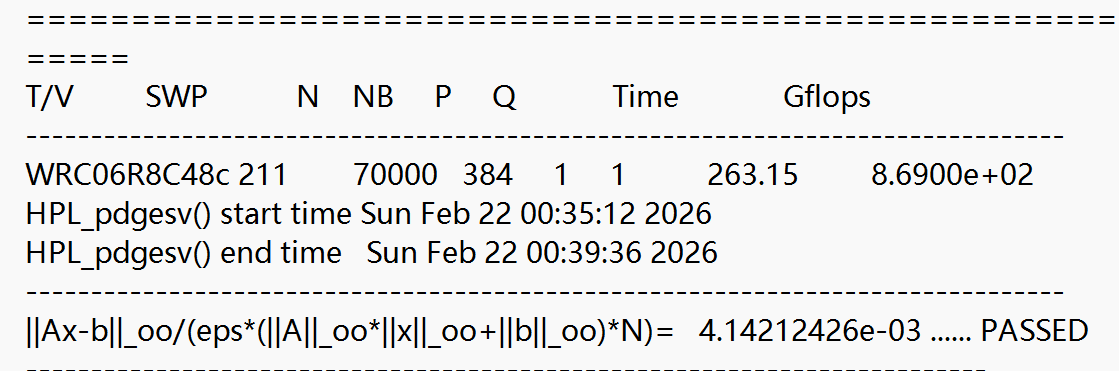
\includegraphics[width=0.8\linewidth]{figures/HPLLOG.png}
    \caption{Performance result of the CPU HPL test}
    \label{fig:hpl reult}
\end{figure}



\subsubsection{GPU Evaluation Results}
\ 

First, we configured the HPL test of the GPU based on experience and found that our test results were not good. 
Then considering that we are using AMD processors, we decided to learn the binary packages that AMD uses. 
Figure \ref{fig:hpl gpu reult} shows the best profile for the performance test with $N{=}36864$, $NB{=}1024$, $P\times Q{=}1\times1$.
Finally, we can get the efficiency is
\begin{equation}
    \text{Efficiency} {=}\frac{\text{Peak of HPL}}{\text{Theoretical Peak }} {=}\frac{\text{632.1 Gflops}}{\text{689 Gflops  }}{\approx}91.74\%
\end{equation}

\begin{figure}[!htb]
    \centering
    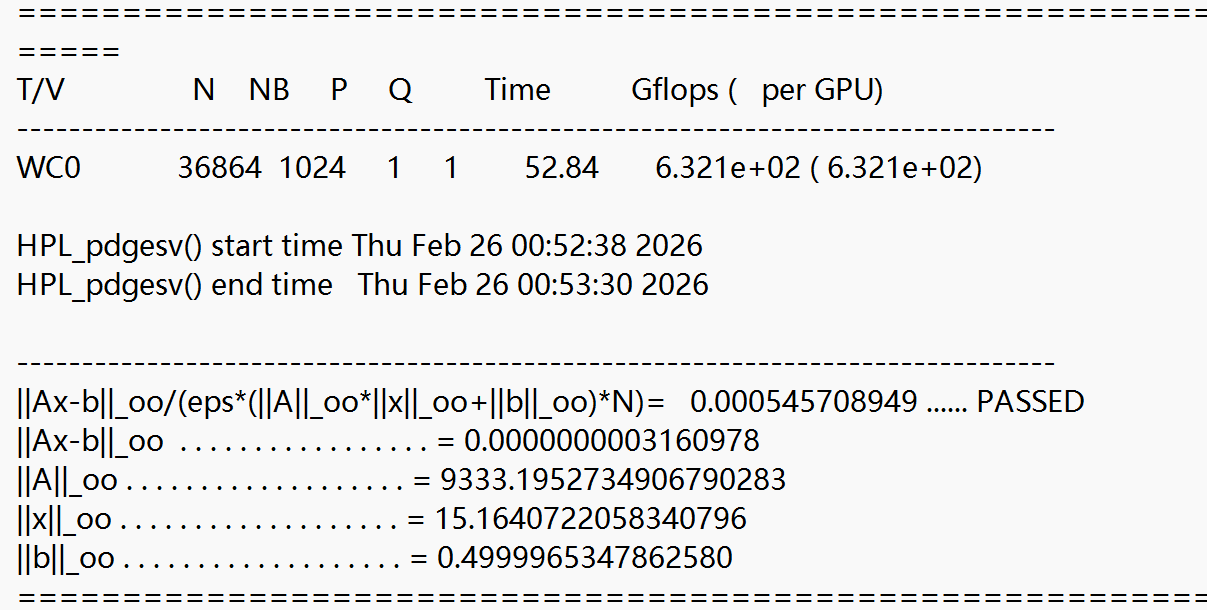
\includegraphics[width=0.8\linewidth]{figures/HPLGPU.png}
    \caption{Performance result of the single GPU HPL test}
    \label{fig:hpl gpu reult}
\end{figure}

\subsection{Summary}
\ 


To sum up, we can see that in HPL testing, in addition parameters $N$, $NB$, $P\times Q$, affecting the test results, different BLAS libraries and compilers perform differently on specific hardware. 
In the end, our \textbf{CPU efficiency and  GPU efficiency all reached about $91.74\%$}.

\clearpage
